\documentclass{beamer}

\usetheme{Warsaw}
\usepackage{graphicx}
\usepackage{ulem}
\usepackage{tikz}
% include.tex
\newcommand{\Bernoulli}[1]{\text{Bernoulli} \left( #1 \right)}
\newcommand{\mydigamma}[1]{\psi \left( #1 \right)}
%\newcommand{\diag}[1]{\text{diag}\left( #1 \right)}
\newcommand{\tr}[1]{\text{tr}\left( #1 \right)}
\newcommand{\Poisson}[1]{\text{Poisson} \left( #1 \right)}
\def \half {\frac{1}{2}}
\def \R {\mathbb{R}}
\def \vbeta {\vec{\beta}}
\def \vy {\vec{y}}
\def \vmu {\vec{\mu}}
\def \vmuqbeta {\vmu_{q(\vbeta)}}
\def \vmubeta {\vmu_{\vbeta}}
\def \Sigmaqbeta {\Sigma_{q(\vbeta)}}
\def \Sigmabeta {\Sigma_{\vbeta}}
\def \va {\vec{a}}
\def \vtheta {\vec{\theta}}
\def \mX {\vec{X}}

\def\ds{{\displaystyle}}

\def\diag{{\mbox{diag}}}


\usepackage{latexsym,amssymb,amsmath,amsfonts}
%\usepackage{tabularx}
\usepackage{theorem}
\usepackage{verbatim,array,multicol,palatino}
\usepackage{graphicx}
\usepackage{graphics}
\usepackage{fancyhdr}
\usepackage{algorithm,algorithmic}
\usepackage{url}
%\usepackage[all]{xy}



\def\approxdist{\stackrel{{\tiny \mbox{approx.}}}{\sim}}
\def\smhalf{\textstyle{\frac{1}{2}}}
\def\vxnew{\vx_{\mbox{{\tiny new}}}}
\def\bib{\vskip12pt\par\noindent\hangindent=1 true cm\hangafter=1}
\def\jump{\vskip3mm\noindent}
\def\etal{{\em et al.}}
\def\etahat{{\widehat\eta}}
\def\thick#1{\hbox{\rlap{$#1$}\kern0.25pt\rlap{$#1$}\kern0.25pt$#1$}}
\def\smbbeta{{\thick{\scriptstyle{\beta}}}}
\def\smbtheta{{\thick{\scriptstyle{\theta}}}}
\def\smbu{{\thick{\scriptstyle{\rm u}}}}
\def\smbzero{{\thick{\scriptstyle{0}}}}
\def\boxit#1{\begin{center}\fbox{#1}\end{center}}
\def\lboxit#1{\vbox{\hrule\hbox{\vrule\kern6pt
      \vbox{\kern6pt#1\kern6pt}\kern6pt\vrule}\hrule}}
\def\thickboxit#1{\vbox{{\hrule height 1mm}\hbox{{\vrule width 1mm}\kern6pt
          \vbox{\kern6pt#1\kern6pt}\kern6pt{\vrule width 1mm}}
               {\hrule height 1mm}}}


%\sloppy
%\usepackage{geometry}
%\geometry{verbose,a4paper,tmargin=20mm,bmargin=20mm,lmargin=40mm,rmargin=20mm}


%%%%%%%%%%%%%%%%%%%%%%%%%%%%%%%%%%%%%%%%%%%%%%%%%%%%%%%%%%%%%%%%%%%%%%%%%%%%%%%%
%
% Some convenience definitions
%
% \bf      -> vector
% \sf      -> matrix
% \mathcal -> sets or statistical
% \mathbb  -> fields or statistical
%
%%%%%%%%%%%%%%%%%%%%%%%%%%%%%%%%%%%%%%%%%%%%%%%%%%%%%%%%%%%%%%%%%%%%%%%%%%%%%%%%

% Sets or statistical values
\def\sI{{\mathcal I}}                            % Current Index set
\def\sJ{{\mathcal J}}                            % Select Index set
\def\sL{{\mathcal L}}                            % Likelihood
\def\sl{{\ell}}                                  % Log-likelihood
\def\sN{{\mathcal N}}                            
\def\sS{{\mathcal S}}                            
\def\sP{{\mathcal P}}                            
\def\sQ{{\mathcal Q}}                            
\def\sB{{\mathcal B}}                            
\def\sD{{\mathcal D}}                            
\def\sT{{\mathcal T}}
\def\sE{{\mathcal E}}                            
\def\sF{{\mathcal F}}                            
\def\sC{{\mathcal C}}                            
\def\sO{{\mathcal O}}                            
\def\sH{{\mathcal H}} 
\def\sR{{\mathcal R}}                            
\def\sJ{{\mathcal J}}                            
\def\sCP{{\mathcal CP}}                            
\def\sX{{\mathcal X}}                            
\def\sA{{\mathcal A}} 
\def\sZ{{\mathcal Z}}                            
\def\sM{{\mathcal M}}                            
\def\sK{{\mathcal K}}     
\def\sG{{\mathcal G}}                         
\def\sY{{\mathcal Y}}                         
\def\sU{{\mathcal U}}  


\def\sIG{{\mathcal IG}}                            


\def\cD{{\sf D}}
\def\cH{{\sf H}}
\def\cI{{\sf I}}

% Vectors
\def\vectorfontone{\bf}
\def\vectorfonttwo{\boldsymbol}
\def\va{{\vectorfontone a}}                      %
\def\vb{{\vectorfontone b}}                      %
\def\vc{{\vectorfontone c}}                      %
\def\vd{{\vectorfontone d}}                      %
\def\ve{{\vectorfontone e}}                      %
\def\vf{{\vectorfontone f}}                      %
\def\vg{{\vectorfontone g}}                      %
\def\vh{{\vectorfontone h}}                      %
\def\vi{{\vectorfontone i}}                      %
\def\vj{{\vectorfontone j}}                      %
\def\vk{{\vectorfontone k}}                      %
\def\vl{{\vectorfontone l}}                      %
\def\vm{{\vectorfontone m}}                      % number of basis functions
\def\vn{{\vectorfontone n}}                      % number of training samples
\def\vo{{\vectorfontone o}}                      %
\def\vp{{\vectorfontone p}}                      % number of unpenalized coefficients
\def\vq{{\vectorfontone q}}                      % number of penalized coefficients
\def\vr{{\vectorfontone r}}                      %
\def\vs{{\vectorfontone s}}                      %
\def\vt{{\vectorfontone t}}                      %
\def\vu{{\vectorfontone u}}                      % Penalized coefficients
\def\vv{{\vectorfontone v}}                      %
\def\vw{{\vectorfontone w}}                      %
\def\vx{{\vectorfontone x}}                      % Covariates/Predictors
\def\vy{{\vectorfontone y}}                      % Targets/Labels
\def\vz{{\vectorfontone z}}                      %

\def\vone{{\vectorfontone 1}}
\def\vzero{{\vectorfontone 0}}

\def\valpha{{\vectorfonttwo \alpha}}             %
\def\vbeta{{\vectorfonttwo \beta}}               % Unpenalized coefficients
\def\vgamma{{\vectorfonttwo \gamma}}             %
\def\vdelta{{\vectorfonttwo \delta}}             %
\def\vepsilon{{\vectorfonttwo \epsilon}}         %
\def\vvarepsilon{{\vectorfonttwo \varepsilon}}   % Vector of errors
\def\vzeta{{\vectorfonttwo \zeta}}               %
\def\veta{{\vectorfonttwo \eta}}                 % Vector of natural parameters
\def\vtheta{{\vectorfonttwo \theta}}             % Vector of combined coefficients
\def\vvartheta{{\vectorfonttwo \vartheta}}       %
\def\viota{{\vectorfonttwo \iota}}               %
\def\vkappa{{\vectorfonttwo \kappa}}             %
\def\vlambda{{\vectorfonttwo \lambda}}           % Vector of smoothing parameters
\def\vmu{{\vectorfonttwo \mu}}                   % Vector of means
\def\vnu{{\vectorfonttwo \nu}}                   %
\def\vxi{{\vectorfonttwo \xi}}                   %
\def\vpi{{\vectorfonttwo \pi}}                   %
\def\vvarpi{{\vectorfonttwo \varpi}}             %
\def\vrho{{\vectorfonttwo \rho}}                 %
\def\vvarrho{{\vectorfonttwo \varrho}}           %
\def\vsigma{{\vectorfonttwo \sigma}}             %
\def\vvarsigma{{\vectorfonttwo \varsigma}}       %
\def\vtau{{\vectorfonttwo \tau}}                 %
\def\vupsilon{{\vectorfonttwo \upsilon}}         %
\def\vphi{{\vectorfonttwo \phi}}                 %
\def\vvarphi{{\vectorfonttwo \varphi}}           %
\def\vchi{{\vectorfonttwo \chi}}                 %
\def\vpsi{{\vectorfonttwo \psi}}                 %
\def\vomega{{\vectorfonttwo \omega}}             %


% Matrices
%\def\matrixfontone{\sf}
%\def\matrixfonttwo{\sf}
\def\matrixfontone{\bf}
\def\matrixfonttwo{\boldsymbol}
\def\mA{{\matrixfontone A}}                      %
\def\mB{{\matrixfontone B}}                      %
\def\mC{{\matrixfontone C}}                      % Combined Design Matrix
\def\mD{{\matrixfontone D}}                      % Penalty Matrix for \vu_J
\def\mE{{\matrixfontone E}}                      %
\def\mF{{\matrixfontone F}}                      %
\def\mG{{\matrixfontone G}}                      % Penalty Matrix for \vu
\def\mH{{\matrixfontone H}}                      %
\def\mI{{\matrixfontone I}}                      % Identity Matrix
\def\mJ{{\matrixfontone J}}                      %
\def\mK{{\matrixfontone K}}                      %
\def\mL{{\matrixfontone L}}                      % Lower bound
\def\mM{{\matrixfontone M}}                      %
\def\mN{{\matrixfontone N}}                      %
\def\mO{{\matrixfontone O}}                      %
\def\mP{{\matrixfontone P}}                      %
\def\mQ{{\matrixfontone Q}}                      %
\def\mR{{\matrixfontone R}}                      %
\def\mS{{\matrixfontone S}}                      %
\def\mT{{\matrixfontone T}}                      %
\def\mU{{\matrixfontone U}}                      % Upper bound
\def\mV{{\matrixfontone V}}                      %
\def\mW{{\matrixfontone W}}                      % Variance Matrix i.e. diag(b'')
\def\mX{{\matrixfontone X}}                      % Unpenalized Design Matrix/Nullspace Matrix
\def\mY{{\matrixfontone Y}}                      %
\def\mZ{{\matrixfontone Z}}                      % Penalized Design Matrix/Kernel Space Matrix

\def\mGamma{{\matrixfonttwo \Gamma}}             %
\def\mDelta{{\matrixfonttwo \Delta}}             %
\def\mTheta{{\matrixfonttwo \Theta}}             %
\def\mLambda{{\matrixfonttwo \Lambda}}           % Penalty Matrix for \vnu
\def\mXi{{\matrixfonttwo \Xi}}                   %
\def\mPi{{\matrixfonttwo \Pi}}                   %
\def\mSigma{{\matrixfonttwo \Sigma}}             %
\def\mUpsilon{{\matrixfonttwo \Upsilon}}         %
\def\mPhi{{\matrixfonttwo \Phi}}                 %
\def\mOmega{{\matrixfonttwo \Omega}}             %
\def\mPsi{{\matrixfonttwo \Psi}}                 %

\def\mone{{\matrixfontone 1}}
\def\mzero{{\matrixfontone 0}}

% Fields or Statistical
\def\bE{{\mathbb E}}                             % Expectation
\def\bP{{\mathbb P}}                             % Probability
\def\bR{{\mathbb R}}                             % Reals
\def\bI{{\mathbb I}}                             % Reals
\def\bV{{\mathbb V}}                             % Reals

\def\vX{{\vectorfontone X}}                      % Targets/Labels
\def\vY{{\vectorfontone Y}}                      % Targets/Labels
\def\vZ{{\vectorfontone Z}}                      %

% Other
\def\etal{{\em et al.}}
\def\ds{\displaystyle}
\def\d{\partial}
\def\diag{\text{diag}}
%\def\span{\text{span}}
\def\blockdiag{\text{blockdiag}}
\def\tr{\text{tr}}
\def\RSS{\text{RSS}}
\def\df{\text{df}}
\def\GCV{\text{GCV}}
\def\AIC{\text{AIC}}
\def\MLC{\text{MLC}}
\def\mAIC{\text{mAIC}}
\def\cAIC{\text{cAIC}}
\def\rank{\text{rank}}
\def\MASE{\text{MASE}}
\def\SMSE{\text{SASE}}
\def\sign{\text{sign}}
\def\card{\text{card}}
\def\notexp{\text{notexp}}
\def\ASE{\text{ASE}}
\def\ML{\text{ML}}
\def\nullity{\text{nullity}}

\def\logexpit{\text{logexpit}}
\def\logit{\mbox{logit}}
\def\dg{\mbox{dg}}

\def\Bern{\mbox{Bernoulli}}
\def\sBernoulli{\mbox{Bernoulli}}
\def\sGamma{\mbox{Gamma}}
\def\sInvN{\mbox{Inv}\sN}
\def\sNegBin{\sN\sB}

\def\dGamma{\mbox{Gamma}}
\def\dInvGam{\mbox{Inv}\Gamma}

\def\Cov{\mbox{Cov}}
\def\Mgf{\mbox{Mgf}}

\def\mis{{mis}} 
\def\obs{{obs}}

\def\argmax{\operatornamewithlimits{\text{argmax}}}
\def\argmin{\operatornamewithlimits{\text{argmin}}}
\def\argsup{\operatornamewithlimits{\text{argsup}}}
\def\arginf{\operatornamewithlimits{\text{arginf}}}


\def\minimize{\operatornamewithlimits{\text{minimize}}}
\def\maximize{\operatornamewithlimits{\text{maximize}}}
\def\suchthat{\text{such that}}


\def\relstack#1#2{\mathop{#1}\limits_{#2}}
\def\sfrac#1#2{{\textstyle{\frac{#1}{#2}}}}


\def\comment#1{
\vspace{0.5cm}
\noindent \begin{tabular}{|p{14cm}|}  
\hline #1 \\ 
\hline 
\end{tabular}
\vspace{0.5cm}
}


\def\mytext#1{\begin{tabular}{p{13cm}}#1\end{tabular}}
\def\mytextB#1{\begin{tabular}{p{7.5cm}}#1\end{tabular}}
\def\mytextC#1{\begin{tabular}{p{12cm}}#1\end{tabular}}

\def\jump{\vskip3mm\noindent}

\def\KL{\text{KL}}
\def\N{\text{N}}
\def\Var{\text{Var}}

\def \E {\mathbb{E}}
\def \BigO {\text{O}}
\def \IG {\text{IG}}
\def \Beta {\text{Beta}}



\usefonttheme{serif}

\title{Troll you a Erik for great good OR How I learned to stop worrying and love floating point numbers}
\author{Mark Greenaway \\ PhD candidate \\ markg@maths.usyd.edu.au}

\mode<presentation>
{ \usetheme{boxes} }

\begin{document}
\begin{frame}
\maketitle
\end{frame}

% Abstract:

% In this talk we will construct the natural numbers, the integers and the rational numbers. We will then
% discuss the fact that the rational numbers are not complete, but have ``holes'', motivating the construction
% of the real numbers. It will be shown that while the rational numbers are countable, the real numbers are not.
% This forces us to approximate if we wish to perform calculations on a finite memory computer in finite time.

% The three major approaches to this problem will be introduced - fixed point, floating point and arbitrary
% precision. Of these, floating point is the one most programmers are likely to first encounter, and the one
% implemented in hardware that you can actually buy today. We will discuss the floating point numbers, along
% with the implications of their definition using some elementary results from numerical analysis. We will also
% discuss alternative representations, particularly arbitrary precision, along with their benefits and
% drawbacks. Some interesting work from the Haskell community in this area will be discussed, including recent
% work by Edward Kmett.

% As mathematics is not a spectator sport, all major results will be proven, assuming only the ZFC axioms. This
% talk will be accessible to anyone with a basic knowledge of high school mathematics and an inquiring mind.

\begin{frame}{Who am I, and why am I here?}
\begin{itemize}
\item Who am I?
\begin{itemize}
\item Did computer science first, then worked as a programmer for a while. Got bored.\\
\note{After I got bored, I went back to Uni to study pure mathematics and statistics. I wanted to get away from computers. Oops.}
\item Third year PhD student in mathematical statistics at the University of Sydney with Dr John Ormerod, working 
in the field of variational approximations to Bayesian models. I'm a computational statistician.\\
\item I could be described as one of those data scientist people. What does that mean? You tell me and we'll
\emph{both} know \ldots
\end{itemize}

\item Why am I here?
\begin{itemize}
\item A few years ago, Erik got really into Haskell.\\
\item Like a good friend, I trolled him about it.\\
\item He said ``Well, if you haven't seriously tried it, how can you know whether it's
any good or not?''.\\
\item So I did. And here I am.
\end{itemize}
\end{itemize}
\end{frame}

\begin{frame}{Mathematics}
\begin{itemize}
\item A lot of people in the functional programming community like algebra, discrete maths, number theory and 
category theory. You draw lots of arrows and form equations.
\item My heart beats for mathematical analysis, statistics and numerical analysis, which have a very different mathematical flavour.
We form inequalities, take limits and approximate when we have no other choice.
\item Mathematicians do not restrict themselves to thinking about things which are computable! \note{That would take all the fun out of life.}
\item Mathematics is not a spectator sport and rests on proof. We will prove every major result this evening for which proofs are available.
\item I assume nothing beyond Year 10 mathematics, but the definitions will come
thick and fast. I hope you've got your thinking caps on!\\
\end{itemize}
\end{frame}

% I want to cover how numbers are constructed, starting from the natural numbers up to the integers, the
% rationals and then the real and complex numbers.

% Because mathematics is \emph{not} a spectator sport, I will be doing this with proofs, live, on the
% whiteboard.

% I'm willing to spend a little bit of time on foundational issues, but not a lot. I'm a mathematical
% analysis/mathematical statistician. There are certain things we accept without question. For instance, most
% mathematicians accept that

% \begin{equation*}
% \mathbb{N} \subset \mathbb{Z} \subset \mathbb{R} \subset \mathbb{C}
% \end{equation*}

% but Liam, Tran's boyfriend, doesn't. He claims that the statement doesn't type check, and hence is
% meaningless. I suspect he's trolling/showing off his superior type theory knowledge, but have been unable to
% pin him down on the issue. Virtually no practicing mathematician would accept this argument. But I'm not a
% type theorist or a Haskell programmer, so my perspective is different. I don't give a flying fuck whether
% things type check, or are even computable. And neither do most pure mathematicians. We work with non-
% computable things all the time. It doesn't trouble us.

% Like the reals. I'm going to present one proof that the reals are uncountable, my favorite one which I learned
% in my third year measure theory course. It's relatively elementary. I'm introducing it because it shows that
% you can't possibly compute with the reals on a computer with finite memory in finite time.

% I'm also going to include a proof that you need the irrational numbers to complete the reals, using the
% square root of 2, although $\pi$ would work just as well.

\begin{frame}{A whirlwind introduction to set theory}
$\forall x$ means for all $x$.\\
Let $A$ and $B$ be sets.\\
To avoid set paradoxes, a set can contain anything except itself.\\
In particular, sets can contain numbers, and other sets.\\
$a \in A$ means the element $a$ is in the set A.\\
$a \notin A$ means the element $a$ is not in the set A.\\
$A \subset B \Leftrightarrow \forall a \in A, a \in B$\\
$A = B \Leftrightarrow A \subset B \text{ and } B \subset A$\\
$A \subseteq B \Leftrightarrow A \subset B \text{ or } A = B$\\
$A \cup B = \{x | x \in A \text{ or } x \in B\}$\\
$A \cap B = \{x | x \in A \text{ and } x \in B\}$\\
Foundational issues are left to logicians and type theorists. Ask Liam O'Connor!
\end{frame}

\def \succ {\text{succ}}
\begin{frame}{Constructing the natural numbers, the integers and the rationals}
There are many possible constructions of the natural numbers. This is the standard one.\\
Let $0 = \emptyset$. \\
Define a successor function $\succ{(x)} = x \cup \{ x \}$.\\
Then\\
$1 = \succ(0) = \succ(\emptyset) = \emptyset \cup \{ \emptyset \} = \{\emptyset\} = \{ 0 \}$.\\
$2 = \succ(1) = \succ(\{ 0 \}) = \{ 0 \} \cup \{ \{ 0 \} \} = \{ 0, \{ 0 \} \} = \{0, 1\}$ and so on.
The integers can then be defined as ordered pairs of the form $(s, x)$ where $s \in \{-, +\}$ and
$x \in \mathbb{N}$. \\
The rational numbers are ratios of integers $a / b$ where $\text{gcd}(a, b) = 1$ i.e. that $a$ and $b$ are
co-prime. Integer multiples i.e. $(k a) / (k b)$ are considered to be equivalent to $a / b$.
\end{frame}


\begin{frame}{The rational numbers are countable}
Proof\\
Construct a list of all the rational numbers
\begin{equation*}
\begin{array}{llll}
1/1,\\
1/2,\\
1/3,& 2/3,\\
1/4,& 2/4,& 3/4,\\
\vdots & \vdots & \vdots & \ddots
\end{array}
\end{equation*}
Then you can see that by going across each row, we can enumerate all of them. Thus we have a bijection between the
natural numbers and the rationals.\\
To do the same for the positive and negative rationals is quite straightforward, and is left as an exercise
for the reader.
\end{frame}

\begin{frame}{But they're full of holes\ldots}
There exist many irrational numbers e.g. $\sqrt{2} \notin \mathbb{Q}$. \\
Proof:
We proceed by contradiction. Assume that $\sqrt{2} \in \mathbb{Q}$. Then $p / q = \sqrt{2}$, for $p, q \in \mathbb{N}$. \\
So $(p^2 / q^2) = 2$ and $p^2 = 2 q^2$. Thus $p^2$ must be even. An even number squared gives
another even number, and an odd number squared gives an odd number. So $q^2$ must be even too, and
hence $p^2$ is divisible by 4, which means that $p$ is divisible by 2. But by the definition of the 
rational numbers, $gcd(p, q) = 1$. Contradiction. Hence $\sqrt{2}$ is irrational.$\Box$\\
Consider the set\\
$S = \{ x \in \mathbb{Q} | x^2 \leq 2 \} = \mathbb{Q} \cap (-\sqrt{2}, \sqrt{2})$.\\
This set clearly includes all of the rational numbers below $\sqrt{2}$. But as we showed above, $\sqrt{2}$
is irrational, so the upper bound $\sqrt{2}$ is not within this set.\\
Thus the rational numbers are full of holes like this.
\end{frame}

\begin{frame}{The reals are trickier to construct. But they're continuous/have no holes}
\begin{itemize}
\item A real number x is called an upper bound for $S$ if $x \geq s$ for all $s \in S$. \\
\item A real number $x$ is the least upper bound (or \emph{supremum}) for $S$ if $x$ is an upper bound for $S$ and $x \leq y$ for every upper bound $y$ of $S$.\\
\item The least-upper-bound property of the reals states that any non-empty set of real numbers that has an upper bound must have a least upper bound in real numbers.
\end{itemize}
The supremum of $S$ above is $\sqrt{2}$, which is in the reals by the least upper bound property.\\
This can be shown to be equivalent to every convergent sequence of real numbers converging within the
real numbers. Thus the real numbers form a complete, ordered field. There are no holes!
\end{frame}

\begin{frame}{But the real numbers aren't countable}
The unit interval $[0, 1]$ is uncountable. \\
Proof:
We proceed by contradiction. Assume that the real numbers were countable.
Enumerate the numbers $a_n$. Furthermore, denote the $m-th$ digit of the $n-th$ number $a_{n, m}.$
All of these numbers are of the form $a_n = 0.a_{n, 1} a_{n, 2} \ldots a_{n, m} \ldots$.
Then construct a number $d = 0.d_1 d_2 d_3 \ldots$ where $d_1 \ne a_{1, 1}$, $d_2 \ne a_{2, 2}$ and
so on.\\
i.e.
\begin{equation*}
\begin{array}{llllll}
a_{1} &= 0.\emph{a_{11}} &a_{12} &a_{13} &a_{14} \ldots \\
a_{2} &= 0.a_{21} &\emph{a_{22}} &a_{23} &a_{24} \ldots \\
a_{2} &= 0.a_{21} &a_{22} &\emph{a_{23}} &a_{24} \ldots \\
a_{2} &= 0.a_{21} &a_{22} &a_{23} &\emph{a_{24}} \ldots \\
\vdots
\end{array}
\end{equation*}
Choose $d$ with the $n-th$ digits not equal to $a_{n n}$ so that it differs from every number on your
list by one digit. Thus $d$ cannot be in your list! Contradiction.
\end{frame}

% The reals not being computable mean that we must adopt some finite approximation of the reals, and compute
% with that. The dominant choice that most people will work with is the floating point numbers. They're
% ubiquitous, and implemented in hardware (CPUs and GPUs). There's a strong body of research work from the
% numerical analysis community on how to compute with them well i.e. to minimise the error. That doesn't make
% them ideal for all purposes. There are many alternative choices which one could make e.g. fixed point, unums,
% arbitrary precision, http://math.andrej.com/2007/09/18/the-role-of-the-interval-domain-in-modern-exact-real-
% airthmetic/, that exact real number computing PhD thesis that Edward Kmett implemented in Haskell etc. I want
% to briefly touch on some of these things, with reference to Amdahl's Law ``the fast drove out the slow, even
% though the fast was slightly wrong'', the Wrath of Kahan (the inventor of floating point is good at showing
% that competing schemes suffer from the same or even worse problems, and generally publishes the results) and
% simple practicality (upon hearing of unums, one of Intel's VPs simply said ``You can't boil the ocean.'' by
% which he meant that expecting people to change every CPU and piece of software in existence to suit your new
% idea is just too large a task, and unrealistic).

% I'm going to talk primarily about floating point, because that's the representation I work with and the one I
% know the most about. It's also the one that most people will encounter and try first. Usually, people swear
% and give up and use something else only when they've tried the floating point numbers and had them not work.

% I want to give a flavour for what numerical analysis is about, why we need it and what we can learn from it.
% I'm particularly looking forward to showing that the floating point numbers do not form a monoid under
% addition, or any other binary operation. I'll then talk about what to do about that i.e. which ordering is
% the optimal ordering to minimise the error in your calculations. There will always be \emph{some} error, but
% we do our best.

% I'll also throw in a couple of jokes that I hope people will like. And I'll talk about myself just a little,
% and how I came to be interested in these things.

\begin{frame}{How do we compute with reals on a finite memory computer in finite time?}
Blunt answer: You don't.
\begin{itemize}
\item We want to be able to compute with the real numbers or something like them on finite memory computers and 
have our calculations complete in finite time. This forces us to approximate. That is, we must introduce
some \emph{error}. \\
\item There are many ways that one might choose to do this. Typically we use a subset of
the rational numbers. \\
\item The dominant choice is the floating point numbers, in particular IEEE 754. \\
\item Other choices include fixed point, arbitrary precision and exotic choices like Unums.
\end{itemize}
\end{frame}

% \begin{frame}{Floating point}
% $\text{sign} \text{mantissa} \times \text{base}^\text{exponent}$ Inf NaN
% Ubiquitous, implemented in hardware you can actually buy off the shelf.
% Numerical analysis
% \end{frame}

% \begin{frame}{The floating point numbers do not form a field!}
% In particular, floating point addition is not associative i.e. $(a + b) + c \ne a + (b + c)$. \\
% \note{Proof: Add a large number to a small number, then add that to another small number.
% Compare to adding two small numbers on the right hand side, then adding the result to the large number.
% You'll lose less precision the second time around. \\
% The functional programming community is interested in algebraic structure. Unfortunately, the floating
% point numbers do not form a monoid under addition, or any other binary arithmetic operation. \
% This has important consequences. If you add a large number to a small number, the large number tends to win
% and the small number loses precision in the sum. \\
% This upsets some people. A lot of things about floating point numbers upset some people. Occasionally, they
% upset me, but the prospect of unemployment or, even worse, having to spend the rest of my life surrounded by
% the sort of person who doesn't believe in real numbers upset me more. \\
% To Do: Proof of numerical analysis showing the best way to add numbers. Sort first, then add from smallest to
% largest.
% }
% \end{frame}

\begin{frame}{The floating point numbers}
Let $\beta=\text{a positive integer}$, the base of our number system. Typically $\beta=2$ or $\beta=16$.
Suppose a number $x$ has exact base representation
\begin{equation*}
x = (\pm 0.\alpha_1 \alpha_2 \alpha_3 \ldots \alpha_t \alpha_{t+1} \ldots) \beta^m = \pm q \beta^m,
\end{equation*}
where $q$ is the \emph{mantissa}, $\beta$ is the \emph{base}, $m$ is the \emph{exponent}, $1 \leq \alpha_1 \leq \beta - 1$
and $0 \leq \alpha_i \leq \beta - 1$ for $i > 1$.

On a computer, we are restricted to a finite set of \emph{floating point numbers}
$F = F(\beta, t, L, U)$ of the form $x^* = (\pm0.a_1 a_2 \ldots a_t) \beta^m$, where $1 \leq a_1 \beta-1$,
$0 \leq a_i \leq \beta - 1$ for $2 \leq i \leq t$, $L \leq m \leq U$ and $t$ is the number of digits.
\end{frame}

\def\fl{\text{fl}}

\begin{frame}
We define a function $\fl: \mathbb{R} \to F$. We have two choices for how to do this:
\begin{itemize}
\item[Chop] If $|x| = 0.a_1 a_2 a_3 \ldots a_t a_{t+1} \ldots \times \beta^m$ then simply drop all digits
after the $t$-th digits
\begin{equation*}
\fl(x) = \text{sign}(x) (0.a_1 a_2 \ldots a_t) \beta^m
\end{equation*}
\item[Round] $\fl(x)$ is the element of $F$ closest to $x$. If $x$ is equidistant to two elements
of $F$, take element of $F$ which is larger in magnitude. Thus, for rounding, if $|x|$ has base $\beta$
expansion then let
\begin{equation*}
|x| + \half \beta^{-t} \beta^m = (0.a_1^* a_2^* \ldots a_t^* a_{t+1}^*\ldots) \beta^m.
\end{equation*}
Then $\fl(x) = \text{sign}(x) (0.a_1^* a_2^* \ldots a_t^*) \beta^m$.
\end{itemize}
\end{frame}

\begin{frame}{Error bounds on floating point numbers}
Theorem: $|x - \fl(x)| \leq \half |x| \beta^{1-t} p$
where $p=1$ for rounding and $p=2$ for chopping.

Proof: Since $x = (\pm 0.\alpha_1 \alpha_2 \ldots \alpha_t \ldots) \beta^m$, we have
$\beta^{m-1} \leq |x| \leq \beta^m$. In the interval $[\beta^{m-1}, \beta^m]$, the floating point numbers
are evenly spaced with spacing $\beta^{m - t}$. Thus, for chopping,
\begin{equation*}
|x - \fl(x)| \leq \beta^{m - t} = \frac{p}{2} \beta^{m-t}, \text{ (with $p = 2$)}
\end{equation*}
and for rounding
\begin{equation*}
|x - \fl(x)| \leq \beta^{m - t} = \frac{p}{2} \beta^{m-t}, \text{ (with $p = 1$)}.
\end{equation*}
Hence
\begin{equation*}
|x - \fl(x) \leq \frac{p}{2} \beta^{m - t} \leq \frac{p}{2} \beta^{1-t} \beta^{m-1} \leq \half |x| \beta^{1-t} p.
\end{equation*}
\end{frame}

\begin{frame}{Error bounds on floating point arithmetic}
Remark: $\delta = \frac{p}{2} \beta^{1-t}$ is called the \emph{unit roundoff error}.\\
Let $\epsilon = \frac{\fl(x) - x}{x}$. Then $\fl(x) = (1 + \epsilon) x$, where $|\epsilon| \leq \delta$.\\
Theorem: Let $\odot$ denote the operation $+, -, \times \text{ or } \div$, and let $x$ and $y$ be
floating point numbers. Then
\begin{equation*}
\fl(x \odot y) = (x \odot y)(1 + \epsilon), \text{ where } |\epsilon| \leq \delta = \frac{p}{2} \beta^{1-t}.
\end{equation*}
Proof: By the previous theorem,
\begin{equation*}
|x \odot y - \fl(x \odot y)| \leq |x \odot y| \frac{p}{2} \beta^{1-t}.
\end{equation*}
Thus, $-|x \odot y| \frac{p}{2} \beta^{1 - t} \leq x \odot y + \fl(x \odot y) \leq \frac{p}{2} \beta^{1 - t} |x \odot y|$.
Hence
\begin{equation*}
(x \odot y)(1 - \frac{|x \odot y|}{x \odot y} \beta^{1-t}) \leq \fl(x \odot y) \leq (x \odot y)(1 + \frac{|x \odot y|}{x \odot y} \beta^{1-t}).
\end{equation*}
It follows that $\fl(x \odot y) = (1 + \epsilon) (x \odot y)$ where
$|\epsilon| \leq \frac{p}{2} \beta^{1-t} = \delta$.
\end{frame}

\begin{frame}{Floating point addition for two or three summands}
\begin{equation*}
\begin{array}{rl}
\fl(x_1 + x_2) &= \fl(\fl(x_1) + \fl(x_2)) = \fl[x_1(1 + \hat{\epsilon_1)}) + x_2(1 + \hat{\epsilon_2})] \\
&= [x_1 (1 + \hat{\epsilon_1}) + x_2 (1 + \hat{\epsilon_1})] (1 + \epsilon),
\end{array}
\end{equation*}
where
$|\hat{\epsilon_1}| \leq \delta$, $|\hat{\epsilon_2}| \leq \delta$ and $|\epsilon_1| \leq \delta$. Similiarly,
\begin{equation*}
\begin{array}{rl}
\fl(x_1 + x_2 + x_3) &= ((x_1 (1 + \hat{\epsilon_1}) + x_2 (1 + \hat{\epsilon_2}))(1 + \epsilon_1) + \\
& \quad x_3 (1 + \hat{\epsilon_3})(1 + \epsilon_2) \\
& = (\quad x_1 (1 + \hat{\epsilon_1}) (1 + \epsilon_1) (1 + \epsilon_2) \\
	&\qquad + x_2 (1 + \hat{\epsilon_2}) (1 + \epsilon_1) (1 + \epsilon_2)) \\
	&\quad + x_3 (1 + \hat{\epsilon_3}) (1 + \epsilon_2)
\end{array}
\end{equation*}
\end{frame}

\begin{frame}{Generalising to n terms}
Continuing this procedure,
\begin{equation*}
\begin{array}{rl}
\fl(\sum_{i=1}^n x_i) &= \quad x_1 (1 + \hat{\epsilon_1}) \prod_{i=1}^{n-1} (1 + \epsilon_i) \\
&\quad + x_2 (1 + \hat{\epsilon_2}) \prod_{i=1}^{n-1} (1 + \epsilon_i) \\
&\quad + x_3 (1 + \hat{\epsilon_3}) \prod_{i=2}^{n-1} (1 + \epsilon_i) \\
&\quad + x_4 (1 + \hat{\epsilon_4}) \prod_{i=3}^{n-1} (1 + \epsilon_i) \\
&\quad + \ldots + x_n (1 + \hat{\epsilon_n}) (1 + \epsilon_{n-1}) \\
&= \sum_{i=1}^n [x_i (1 + \hat{\epsilon_i}) \prod_{j=1}^{n-1} (1 + \epsilon_j)].
\end{array}
\end{equation*}
Conclusion: 
\begin{itemize}
\item Floating point addition \emph{does not commute}. Neither does any other floating point
operation.
\item Hence the floating point numbers do not form a monoid under addition.\\
\item To reduce rounding error, a sequence should be summed from small numbers to large numbers on a
computer.
\end{itemize}
\end{frame}

\begin{frame}{Looks like this \ldots}
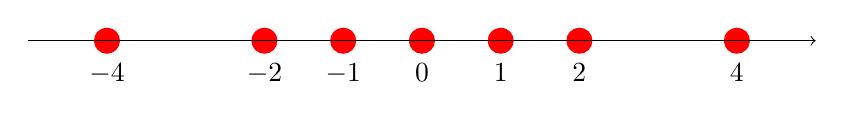
\begin{tikzpicture}
\foreach \x in {-4, -2, -1, 0, 1, 2, 4}
	{\node[circle, minimum size=0.1 cm, fill=red, label = below : {$\x$}] at (\x, 0) {};};
\draw[->] (-5, 0) -- (5, 0);
\end{tikzpicture}
\end{frame}

\begin{frame}{Alternatives to floating point: more precision or arbtitrary precision}
\begin{itemize}
\item The easy answer is to throw more bits at the problem for more precision. Rather than single precision floating point, why not double? Or
quadruple aka double double? Or double double double? Or, well, you get the idea \ldots
\item One alternative from a conceptual standpoint is arbitrary precision, where numbers don't have to be
stored in a fixed amount of memory.
\item Just keep computing with more digits until you reach the desired level of accuracy. You could do this with
streaming.
\item Examples from the Haskell community: Ed Kmett's work, \texttt{mvr}
\end{itemize}
\end{frame}

\begin{frame}{More exotic alternatives: UNums 2.0}
\begin{itemize}
\item Professor Gustaffson, ex-Intel\\
\item Author of ``The End of Error: Unum Computing'', already superceded.\\
\item Abandons previous ideas of floating point representation completely.
\item Key idea:
\begin{equation*}
\text{Let }f(x) = \frac{x}{1 + |x|}.
\end{equation*}
\begin{tikzpicture}
\node (0) at (0, 1) {};
\node (1) at (0, 0) {};
% \draw[->] (B) to [out=0, in = 270] (A);
\path[<-, operation]
(0) edge [bend left] node[below left] {$f$} (1);
\path[<-] (0) edge [bend left] (1);
\path[<-, operation]
(0) edge [bend right] node[below left] {$f$} (1);
\end{tikzpicture}
Clearly $f: (-\infty, \infty) \to (-1, 1)$ and is a bijection from the real line to the open unit interval.\\
% TODO: This would be a nice place for a TikZ diagram of the situation, don't you think?
\item Very new, presented at Multicore World 2016. No proofs in the Powerpoint presentation!\\
\item Lose precision gradually and gracefully, rather than in sudden bursts like floating point.\\
\item A little bird tells me that Intel finds this interesting, and ``may look at implementing this in
six year's time.''. They refused to be quoted!
\end{itemize}
\end{frame}

\begin{frame}{But \ldots}
\begin{itemize}
\item Floating point arithmetic is ubiquitous, like QWERTY, or imperative programming
or \ldots.
\item The Wrath of Kahan: alternatives often end up suffering from the same shortcomings. One of the inventors of
floating point, William Kahan aka the Father of floating point arithmetic, enjoys pointing this out.
\item One clock cycle is about as long as I care to wait.
\item Serious answer: Use the right representation in the right situation. But know what price you're paying 				in terms of both memory and time, and how much precision you're really getting.
\end{itemize}
\end{frame}

% [2:34pm] mvr_: back in the 70's Bill Gosper figured out how to do arithmetic on continued fractions
% [2:35pm] mvr_: what ed and I were doing was basically variations on the theme
% [2:35pm] StyxAlso: That’s pretty interesting.
% [2:37pm] mvr_: also, listening to dibblego talk can be almost unbearable; he seems to not understand that people don't have infinite time to build a whole ecosystem in his favourite language whenever they want to do something simple
% [2:38pm] mvr_: I just hope you don't get the wrong impression about the haskell community from him
% [2:39pm] StyxAlso: Thanks 
% [2:39pm] StyxAlso: I do get that impression from some people in the Haskell community, but certainly not all of them.
% [2:39pm] StyxAlso: And having worked as a computer programmer for nearly a decade, and been pretty unbearable myself at times, I’m used to dealing with unbearable people
% [2:40pm] StyxAlso: Thanks for the validation, though. I was finding that conversation pretty difficult.
% [2:48pm] StyxAlso: My email is certifiedwaif@gmail.com. I’m snowed under today, but could we tee up another time? You sound very clued in about this area 
% [2:49pm] mvr_: I'm actually just a masters student with almost no industry experience
% [2:49pm] mvr_: but my email is mitchell.v.riley@gmail.com if you'd like to know a bit about the CF stuff
% [2:51pm] StyxAlso: ta

% [2:10pm] mvr_: StyxAlso: you may be interested in http://herbie.uwplse.org/ , and the associated GHC plugin
% [2:10pm] HEGX64 joined the chat room.
% [2:11pm] StyxAlso: mvr_: That looks like really nice work.
% [2:11pm] StyxAlso: The blog posts look ideal for improving my presentation. Thank you very much, mvr_.
% [2:11pm] StyxAlso: The person writing that web page seems pro-floating point, which is refreshing.
% [2:12pm] StyxAlso: People often have their own favorite alternative representation e.g. unums, arbitrary precision, that thing that Edward Kmett implemented
% [2:12pm] mankyKitty: haha, I'm not anti-floating point, I'm just floating point averse because I'm an idiot and would rather avoid the pain
% [2:12pm] StyxAlso: They’re usually quick to discuss the advantages, but less willing to discuss the disadvantages
% [2:12pm] mankyKitty:
% [2:13pm] StyxAlso: mankyKitty: Haha, I can’t avoid that pain. I’d have to leave the field 
% [2:14pm] mankyKitty: Then I will defer to your expertise on the matter and look forward to using your library so i can gloat about getting it right without trying. *ahem* 
% [2:14pm] beckyconning_ left the chat room. (Quit: Connection closed for inactivity)
% [2:16pm] mvr_: argh, I swear I beat ed by a week or two on that stuff
% [2:22pm] carter_cloud: StyxAlso: Haskell has a sweet impl of double double precision numbers.  A friend and I are working on getting some of the trig / exp / log funs implemented on it.
% [2:23pm] StyxAlso: carter_cloud: That sounds good. I’d be interested to know about the trade-offs, from a numerical analysis point of view.
% [2:23pm] StyxAlso: mvr_: Maybe you could tell me about it some time? I’d like to include it in my talk.
% [2:24pm] carter_cloud: It has more bits of precision within the representable dynamic range.
% [2:25pm] carter_cloud: Ie every number you rep as the sum of two doubles is exact
% [2:25pm] carter_cloud: Which is a lotta numbers.
% [2:25pm] carter_cloud: So for things that are neither too big not too small you get effectively twice as many bits of precision
% [2:27pm] StyxAlso: That sounds great. Double precision tops out at ~2.2*10^308.
% [2:27pm] StyxAlso: I hit that upper limit all the time working with some functions.
% [2:28pm] carter_cloud: Same dynamic range.  Sorry
% [2:29pm] carter_cloud: You want mpfr if you want both 
% [2:29pm] carter_cloud: Or the numbers package.  Which I now allegedly maintain.
% [2:31pm] StyxAlso:
% [2:31pm] StyxAlso: carter_cloud: Are you in Australia? Or contactable?
% [2:31pm] StyxAlso: as in, via voice.
% [2:31pm] carter_cloud: I'm in NYC.
% [2:32pm] carter_cloud: And yes I can use vid chat stuff.
% [2:32pm] StyxAlso: Great! It’d be interesting to chat to someone about this stuff.
% [2:32pm] carter_cloud: But I'm on the toilet atm. So wait a bit
% [2:32pm] StyxAlso: And you’re still on IRC. How’s that for parallelism?
% [2:34pm] carter_cloud: Async obv
% [2:36pm] carter_cloud: I can chat in 15 I guess
% [2:40pm] StyxAlso: I’m at Uni atm. Would another day be okay for you?
% [2:49pm] carter_cloud: Sure
% [2:50pm] carter_cloud: Or lurk on numerical Haskell
% [2:51pm] StyxAlso: #numerical-haskell on FreeNode?
% [2:52pm] carter_cloud: Mineeee
% [2:52pm] carter_cloud: there can be only one
% [2:53pm] edwardk: StyxAlso: i concede priority to mvr_ with regards to continued fractions. -- afterwards, i had a few novel ideas about weird operadic encodings of linear fractional transformations, but again mvr_ beat me to turning them into actual code.
% [2:54pm] mvr_: edwardk: we never did get that working properly
% [2:54pm] StyxAlso: edwardk: Any advantages/disadvantages of that representation of the reals versus floating point?
% [2:55pm] edwardk: StyxAlso: arbitrary precision that you pay for as you go
% [2:55pm] edwardk: rather than have to start all over again when you find you didn't have enough
% [2:55pm] StyxAlso: So the same caveats as for, say, arbitrary precision with a decimal representation?
% [2:55pm] edwardk: while demanding the optimal amount from each input
% [2:55pm] edwardk: no
% [2:55pm] StyxAlso: Okay. Could you explain the difference to me?
% [2:56pm] edwardk: you might have a representation that says give me n decimal places of precision
% [2:56pm] edwardk: and computes it
% [2:56pm] StyxAlso: Bear in mind, I don’t know continued fractions very well.
% [2:56pm] edwardk: but to do that, you'll usually have to ask for _more_ than n decimal places of precision from your arguments
% [2:56pm] edwardk: so you have to take super-conservative bounds
% [2:57pm] carter_cloud: Where's this code by mvr?
% [2:58pm] mvr_: my attempt at making it runnable is at https://github.com/mvr/fractions
% [2:59pm] erikd: i did a continued fractions thing in ocaml about 10 years ago.
% [2:59pm] StyxAlso: edwardk: So you have to do more computation for the same precision?
% [3:00pm] edwardk: erikd: the code we have isn't about fractions but rather nested linear fractional transformations
% [3:00pm] mvr_: carter_cloud: it was a good experiment, but not pretty so I'd be fine with throwing most of my changes away
% [3:00pm] erikd: ah ok
% [3:00pm] edwardk: StyxAlso: neither side really has a clear advantage on that front, the constants may be worse
% [3:00pm] StyxAlso: Okay. But it’s another option.
% [3:00pm] edwardk: yeah
% [3:00pm] edwardk: its an experiment
% [3:01pm] StyxAlso: And the numerical analysis has been done? i.e. people know how to get the error bounds for various things they may want to compute.
% [3:01pm] mvr_: oh, I meant the stuff I added wasn't pretty
% [3:01pm] edwardk: and there are classes of equations where this form may be a big win over everything i know
% [3:02pm] StyxAlso: Okay.
% [3:02pm] jedws left the chat room. (Read error: Connection reset by peer)
% [3:02pm] edwardk: the numerical analysis of this stuff is based on the same analysis that gave the first serious world record computation of pi to ~17 million digits or so
% [3:02pm] edwardk: so yeah it can handle precision
% [3:02pm] jedws joined the chat room.
% [3:02pm] edwardk: and it can back up the precision of the answer rigorously
% [3:03pm] edwardk: my trick is mostly about trying to avoid having the performance of that degrade so much as the computation gets bigger
% [3:05pm] StyxAlso: Right. Performance is key. The fast tends to drive out the slow, even if the fast is slightly wrong.
\end{document}
